% document.tex
% 请使用最新发行版本的TeX Live编译(编译方式为XeLaTeX)。
\documentclass[master,academic]{ysuthesis} % Use the custom document class
%%%%%%%%%%%%%%%%%%%%%%%%%%%%%%%%%%%%%%%%%%%%%%%%%%%%%%%%%%%%%%%%
%	博士/硕士
%	doctor——博士,中英文对照的图题和表题采用命令\bicaption{中文标题}{英文标题}实现,子图使用命令\bisubcaptionbox{中文标题}{英文标题}[]{}实现。
%	master——硕士(默认选项),中文的图题和表题采用用命令\caption{标题}实现,子图使用命令\subcaptionbox{中文标题}[]{}实现。
%%%%%%%%%%%%%%%%%%%%%%%%%%%%%%%%%%%%%%%%%%%%%%%%%%%%%%%%%%%%%%%%
%   学术学位/专业学位
%	academic——学术学位(默认选项)
%	professional——专业学位
%%%%%%%%%%%%%%%%%%%%%%%%%%%%%%%%%%%%%%%%%%%%%%%%%%%%%%%%%%%%%%%%

%%%%%%%%%%%%%%%%%%%%%%%%%%%%%%%%%%%%%%%%%%%%%%%%%%%%%%%%%%%%%%%%
%	图片路径
\graphicspath{{fig/}}
%%%%%%%%%%%%%%%%%%%%%%%%%%%%%%%%%%%%%%%%%%%%%%%%%%%%%%%%%%%%%%%%

%%%%%%%%%%%%%%%%%%%%%%%%%%%%%%%%%%%%%%%%%%%%%%%%%%%%%%%%%%%%%%%%
%	Document metadata
%%%%%%%%%%%%%%%%%%%%%%%%%%%%%%%%%%%%%%%%%%%%%%%%%%%%%%%%%%%%%%%%
\title{生物同步康复机制理论与应用}{Bio-Syncretic Rehabilitation Mechanism Theory and	Application}
\author{张小明}{Zhang Xiaoming}
\school{电气工程学院}{School of Electrical Engineering}
\subject{电气工程}{Electrical Engineering}
\applydegree{工学}{Engineering}
\supervisor{郭大师}{教授}{Guo Dashi}{Professor}
\assosupervisor{吴高工}{高级工程师}{Wu Gaogong}{Senior Engineer}
\date{2024年6月}{June, 2024}
\bookclassificationnumber{TM464}{621.3}
\security{公开}
\researchtype{产品研发}%产品研发、应用研究、工程设计、基础研究等,学术学位可忽略

\begin{document}

	\makecover

	\cabstract{摘要是论文内容的高度概括,应具有独立性和自含性,即不阅读论文的全文,就能通过摘要了解整个论文的必要信息。摘要应包括本论文研究的目的、理论与实际意义、主要研究内容、研究方法等,重点突出研究成果和结论。
		
		摘要的内容要完整、客观、准确,应做到不遗漏、不拔高、不添加。摘要应按层次逐段简要写出,避免将摘要写成目录式的内容介绍。摘要在叙述研究内容、研究方法和主要结论时,除作者的价值和经验判断可以使用第一人称外,一般使用第三人称,采用“分析了……原因”“认为……”“对……进行了探讨”等记述方法进行描述,避免主观性的评价意见,避免对背景、目的、意义、概念和一般性(常识性)理论叙述过多。
		
		摘要需采用规范的名词术语(包括地名、机构名和人名)。对个别新术语或无中文译文的术语,可用外文或在中文译文后加括号注明外文。摘要中不宜使用公式、化学结构式、图表、非常用的缩写词和非公知公用的符号与术语,不标注引用文献编号。
		
		摘要的字数(以汉字计),硕士学位论文一般为500~650字,博士学位论文为900~1200字,均以能将规定内容阐述清楚为原则,文字要精练,段落衔接要流畅。
		
		……
		}

	\ckeywords{关键词1;关键词2;……;关键词8}

	\eabstract{The rehabilitation mechanism is the foundation for a rehabilitation robot to realize its motion, and the quality of the rehabilitation mechanism decides the rehabilitation effect of patients with the rehabilitation robot. The research of rehabilitation mechanism is the key content in rehabilitation engineering. The bio-syncretic rehabilitation mechanism (BSRM) is a new type of modern mechanism composed of human body and machine, and it can meet the design requirements of rehabilitation robot more effectively because of the interaction and harmonization between human body and machine during the rehabilitation exercise. This paper presents the relative systematic research on BSRM and its application. The main contents of this paper are as follows:

		The concept of rehabilitation mechanism is proposed based on the relationship between human body mechanism and mechanical mechanism in the rehabilitation kinematics system, and the characteristics, degree of freedom, classification and symbol representation of this new kind of mechanism is introduced. The approaches to type synthesis of parallel BSRM and series BSRM are developed based on screw theory and the characteristic of BSRM, and some parallel BSRMs for ankle joint rehabilitation and series BSRMs for knee joint rehabilitation are got.
	}

	\ekeywords{keyword1; keyword2; ……; keyword8}

	\customizedtableofcontents

	\chapter{绪论}

		三四五六七八九〇壹贰叁肆伍陆柒捌玖零一二三四五六七八九〇壹贰叁肆伍陆柒捌玖零一二三四五六七八九〇壹贰叁肆伍陆柒捌玖零一二三四五六七八九〇壹贰叁肆伍陆柒捌玖零一二三四五六七八九〇壹贰叁肆伍陆柒捌玖零

	\section{二级标题1}

		三四五六七八九〇壹贰叁肆伍陆柒捌玖零一二三四五六七八九〇壹贰叁肆伍陆柒捌玖零一二三四五六七八九〇壹贰叁肆伍陆柒捌玖零一二三四五六七八九〇壹贰叁肆伍陆柒捌玖零一二三四五六七八九〇壹贰叁肆伍陆柒捌玖零

	\section{二级标题2}

		三四五六七八九〇壹贰叁肆伍陆柒捌玖零一二三四五六七八九〇壹贰叁肆伍陆柒捌玖零一二三四五六七八九〇壹贰叁肆伍陆柒捌玖零一二三四五六七八九〇壹贰叁肆伍陆柒捌玖零一二三四五六七八九〇壹贰叁肆伍陆柒捌玖零\footnote{党理、科研团队建设、一流课程建设}


	\subsection{三级标题1}

		三四五六七八九〇壹贰叁肆伍陆柒捌玖零一二三四五六七八九〇壹贰叁肆伍陆柒捌玖零一二三四五六七八九〇壹贰叁肆伍陆柒捌玖零一二三四五六七八九〇壹贰叁肆伍陆柒捌玖零一二三四五六七八九〇壹贰叁肆伍陆柒捌玖零

	\subsection{三级标题2}

		三四五六七八九〇壹贰叁肆伍陆柒捌玖零一二三四五六七八九〇壹贰叁肆伍陆柒捌玖零一二三四五六七八九〇壹贰叁肆伍陆柒捌玖零一二三四五六七八九〇壹贰叁肆伍陆柒捌玖零一二三四五六七八九〇壹贰叁肆伍陆柒捌玖零\footnote{党建工作、科研工作、辅导员队伍建设、学科建设等方面的基本情况。在主题党日谋划、学生应急事件处理、科研团队建设、一流课程建设}

	\chapter{第2章标题}

	\section{二级标题}

		学位论文的撰写是一个系统性的研究过程,涉及选择主题、制定研究问题、文献综述、确定研究方法、收集和分析数据、撰写论文、修改审阅等步骤。首先,选择一个具有研究意义和足够研究空间的主题,然后明确研究问题,并进行相关文献综述。确定合适的研究方法后,收集和分析数据,根据结论撰写论文,确保逻辑清晰和论证严谨。最后,进行修改审阅,确保论文质量和完整性。整个过程需要耐心和专注,以确保论文的学术价值和质量。

		学位论文的撰写是一个系统性的研究过程,涉及选择主题、制定研究问题、文献综述、确定研究方法、收集和分析数据、撰写论文、修改审阅等步骤。首先,选择一个具有研究意义和足够研究空间的主题,然后明确研究问题,并进行相关文献综述。确定合适的研究方法后,收集和分析数据,根据结论撰写论文,确保逻辑清晰和论证严谨。最后,进行修改审阅,确保论文质量和完整性。整个过程需要耐心和专注,以确保论文的学术价值和质量。

		学位论文的撰写是一个系统性的研究过程,涉及选择主题、制定研究问题、文献综述、确定研究方法、收集和分析数据、撰写论文、修改审阅等步骤。首先,选择一个具有研究意义和足够研究空间的主题,然后明确研究问题,并进行相关文献综述。确定合适的研究方法后,收集和分析数据,根据结论撰写论文,确保逻辑清晰和论证严谨。最后,进行修改审阅,确保论文质量和完整性。整个过程需要耐心和专注,以确保论文的学术价值和质量。

		学位论文的撰写是一个系统性的研究过程,涉及选择主题、制定研究问题、文献综述、确定研究方法、收集和分析数据、撰写论文、修改审阅等步骤。首先,选择一个具有研究意义和足够研究空间的主题,然后明确研究问题,并进行相关文献综述。确定合适的研究方法后,收集和分析数据,根据结论撰写论文,确保逻辑清晰和论证严谨。最后,进行修改审阅,确保论文质量和完整性。整个过程需要耐心和专注,以确保论文的学术价值和质量。

		学位论文的撰写是一个系统性的研究过程。

		三四五六七八九〇壹贰叁肆伍陆柒捌玖零一二三四五六七八九〇壹贰叁肆伍陆柒捌玖零一二三四五六七八九〇壹贰叁肆伍陆柒捌玖零一二三四五六七八九〇壹贰叁肆伍陆柒捌玖零一二三四五六七八九〇壹贰叁肆伍陆柒捌玖零一二三四五六七八九〇壹贰叁肆伍陆柒捌玖零一二三四五六七八九〇壹贰叁肆伍陆柒捌玖零一二三四五六七八九〇壹贰叁肆伍陆柒捌玖零一二三四五六七八九〇壹贰叁肆伍陆柒捌玖零

		三四五六七八九〇壹贰叁肆伍陆柒捌玖零一二三四五六七八九〇壹贰叁肆伍陆柒捌玖零一二三四五六七八九〇壹贰叁肆伍陆柒捌玖零一二三四五六七八九〇壹贰叁肆伍陆柒捌玖零一二三四五六七八九〇壹贰叁肆伍陆柒捌玖零一二三四五六七八九〇壹贰叁肆伍陆柒捌玖零一二三四五六七八九〇壹贰叁肆伍陆柒捌玖零一二三四五六七八九〇壹贰叁肆伍陆柒捌玖零一二三四五六七八九〇壹贰叁肆伍陆柒捌玖零

		三四五六七八九〇壹贰叁肆伍陆柒捌玖零一二三四五六七八九〇壹贰叁肆伍陆柒捌玖零一二三四五六七八九〇壹贰叁肆伍陆柒捌玖零一二三四五六七八九〇壹贰叁肆伍陆柒捌玖零一二三四五六七八九〇壹贰叁肆伍陆柒捌玖零一二三四五六七八九〇壹贰叁肆伍陆柒捌玖零一二三四五六七八九〇壹贰叁肆伍陆柒捌玖零一二三四五六七八九〇壹贰叁肆伍陆柒捌玖零一二三四五六七八九〇壹贰叁肆伍陆柒捌玖零

		三四五六七八九〇壹贰叁肆伍陆柒捌玖零一二三四五六七八九〇壹贰叁肆伍陆柒捌玖零一二三四五六七八九〇壹贰叁肆伍陆柒捌玖零一二三四五六七八九〇壹贰叁肆伍陆柒捌玖零一二三四五六七八九〇壹贰叁肆伍陆柒捌玖零一二三四五六七八九〇壹贰叁肆伍陆柒捌玖零一二三四五六七八九〇壹贰叁肆伍陆柒捌玖零一二三四五六七八九〇壹贰叁肆伍陆柒捌玖零一二三四五六七八九〇壹贰叁肆伍陆柒捌玖零

		三四五六七八九〇壹贰叁肆伍陆柒捌玖零一二三四五六七八九〇壹贰叁肆伍陆柒捌玖零一二三四五六七八九〇壹贰叁肆伍陆柒捌玖零一二三四五六七八九〇壹贰叁肆伍陆柒捌玖零一二三四五六七八九〇壹贰叁肆伍陆柒捌玖零一二三四五六七八九〇壹贰叁肆伍陆柒捌玖零一二三四五六七八九〇壹贰叁肆伍陆柒捌玖零一二三四五六七八九〇壹贰叁肆伍陆柒捌玖零一二三四五六七八九〇壹贰叁肆伍陆柒捌玖零

		三四五六七八九〇壹贰叁肆伍陆柒捌玖零一二三四五六七八九〇壹贰叁肆伍陆柒捌玖零一二三四五六七八九〇壹贰叁肆伍陆柒捌玖零一二三四五六七八九〇壹贰叁肆伍陆柒捌玖零一二三四五六七八九〇壹贰叁肆伍陆柒捌玖零一二三四五六七八九〇壹贰叁肆伍陆柒捌玖零一二三四五六七八九〇壹贰叁肆伍陆柒捌玖零一二三四五六七八九〇壹贰叁肆伍陆柒捌玖零一二三四五六七八九〇壹贰叁肆伍陆柒捌玖零

		学位论文的撰写是一项系统性的研究过程,包括选择研究主题、明确研究问题、文献综述、确定研究方法、收集和分析数据、撰写论文、修改和审阅等步骤。在撰写过程中,研究者需要深入调查相关文献、运用科学方法进行研究、清晰地表达研究结果和结论,并确保论文的逻辑性和严谨性。最终,论文的质量将受到审稿人和导师的评价,对学位授予具有关键影响。

		文献\cite{texbook,latex:companion,latex2e,knuth:1984,lesk:1977}为参考文献示例\upcite{texbook,latex:companion,latex2e,knuth:1984,lesk:1977}。

		图\ref{fig:ysu_logo}为插入单张图片示例。

		%-------------------插入单张图片示例开始-------------------
			\begin{figure}[!ht]
				\centering
				
\includegraphics[width=2.79in]{ysu_logo}
				\caption{硕士论文图形}
				\label{fig:ysu_logo}
			\end{figure}
		%-------------------插入单张图片示例结束-------------------
			\begin{figure}[!ht]
				\centering
				
\includegraphics[width=0.6\textwidth]{ysu_logo}
				\bicaption{博士论文图形}{A single center graphics A single center graphics }
				\label{ysulogo}
            \end{figure}

		三四五六七八九〇壹贰叁肆伍陆柒捌玖零一二三四五六七八九〇壹贰叁肆伍陆柒捌玖零一二三四五六七八九〇壹贰叁肆伍陆柒捌玖零一二三四五六七八九〇壹贰叁肆伍陆柒捌玖零一二三四五六七八九〇壹贰叁肆伍陆柒捌玖零一二三四五六七八九〇壹贰叁肆伍陆柒捌玖零一二三四五六七八九〇壹贰叁肆伍陆柒捌玖零一二三四五六七八九〇壹贰叁肆伍陆柒捌玖零一二三四五六七八九〇壹贰叁肆伍陆柒捌玖零

		图\ref{fig_ysunationalbase}、图\ref{fig_ysunationalbase}\subref{fig_mmst}、图\ref{fig_ysunationalbase}\subref{fig_finesteel}、图\ref{fig_ysunationalbase}\subref{fig_innovativetalents}和图\ref{fig_ysunationalbase}\subref{fig_coldrolledstrip}为插入多张图片示例。

		%-------------------插入多张图片示例开始-------------------
			\begin{figure}[!ht]
				\centering
				\subcaptionbox{亚稳材料制备技术与科学国家重点实验室\label{fig_mmst}}[0.49\textwidth]{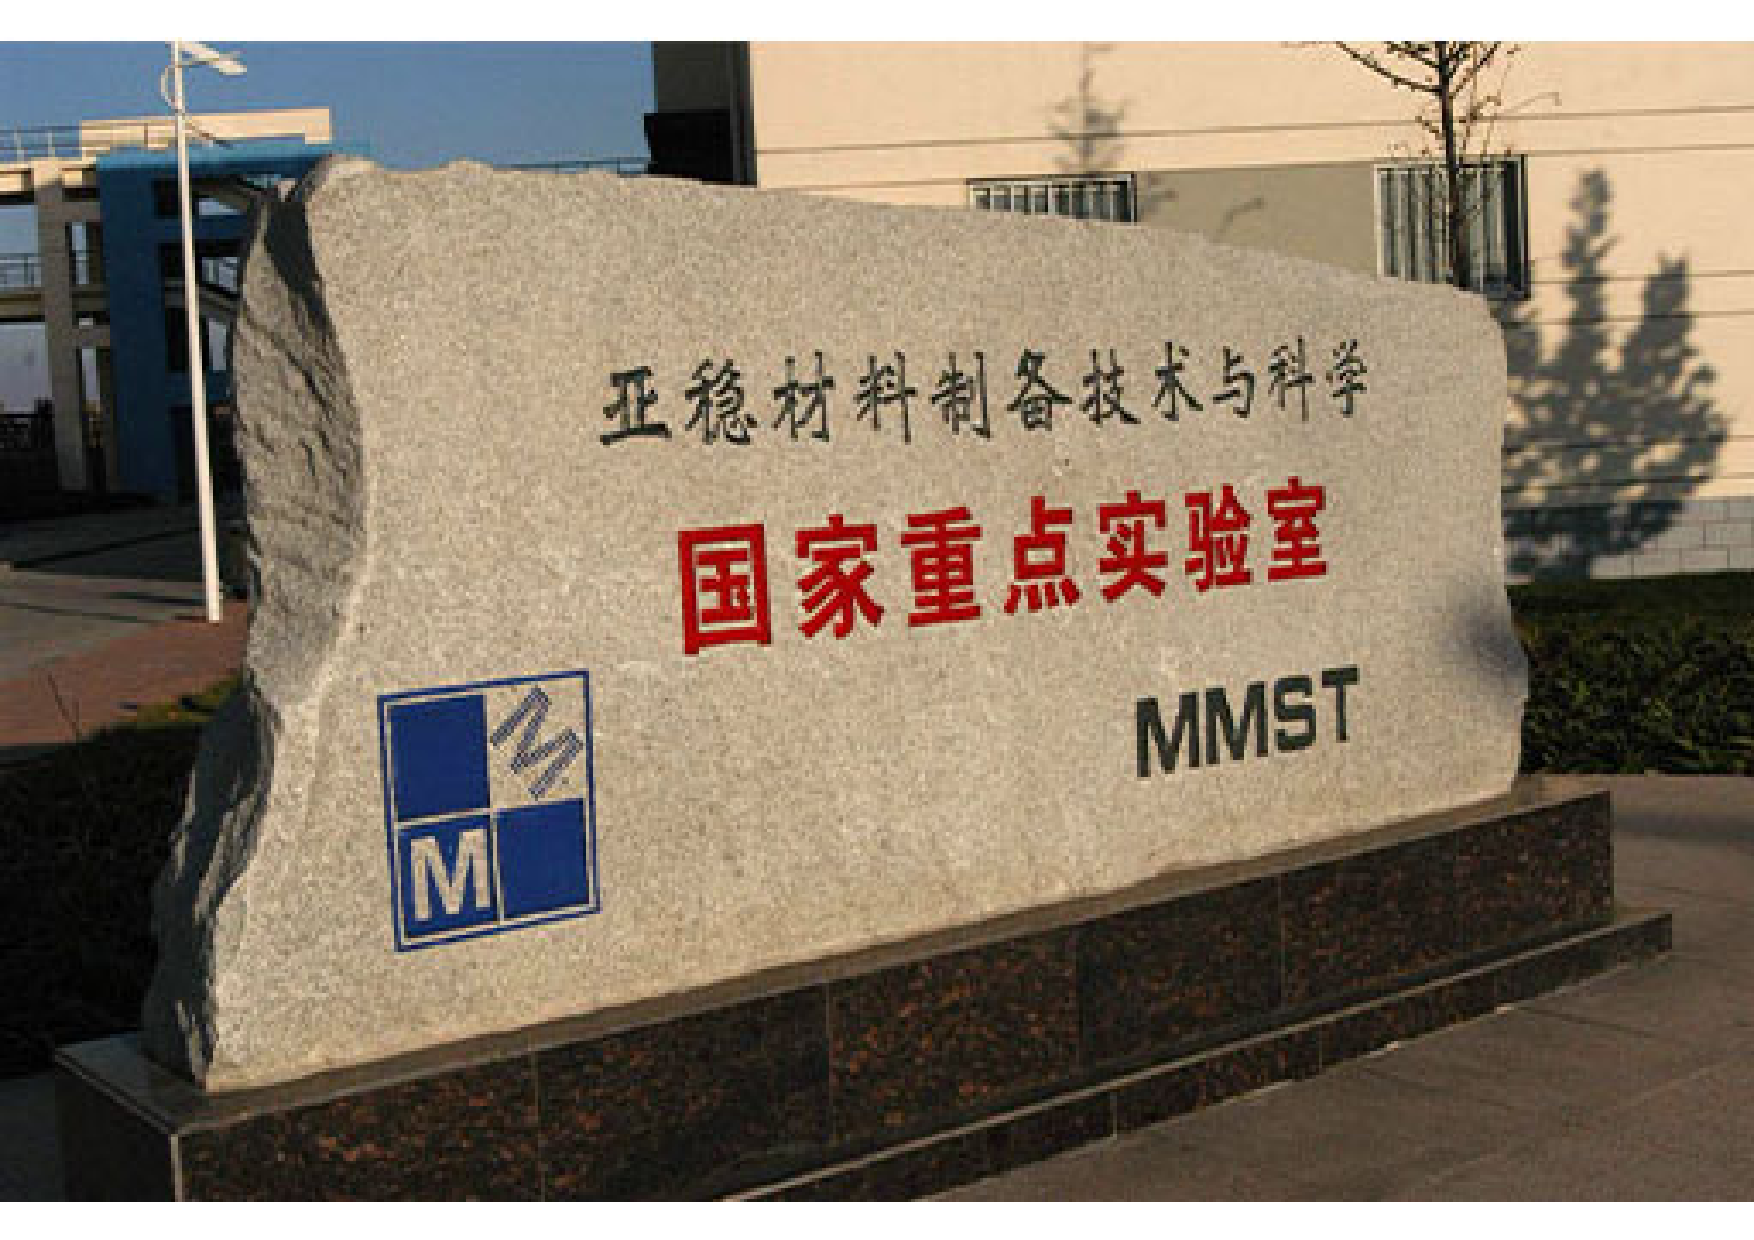
\includegraphics[width=0.4\textwidth]{亚稳材料制备技术与科学国家重点实验室.pdf}}
				\subcaptionbox{精品钢铁生产工艺装备智能化省部共建协同创新中心\label{fig_finesteel}}[0.49\textwidth]{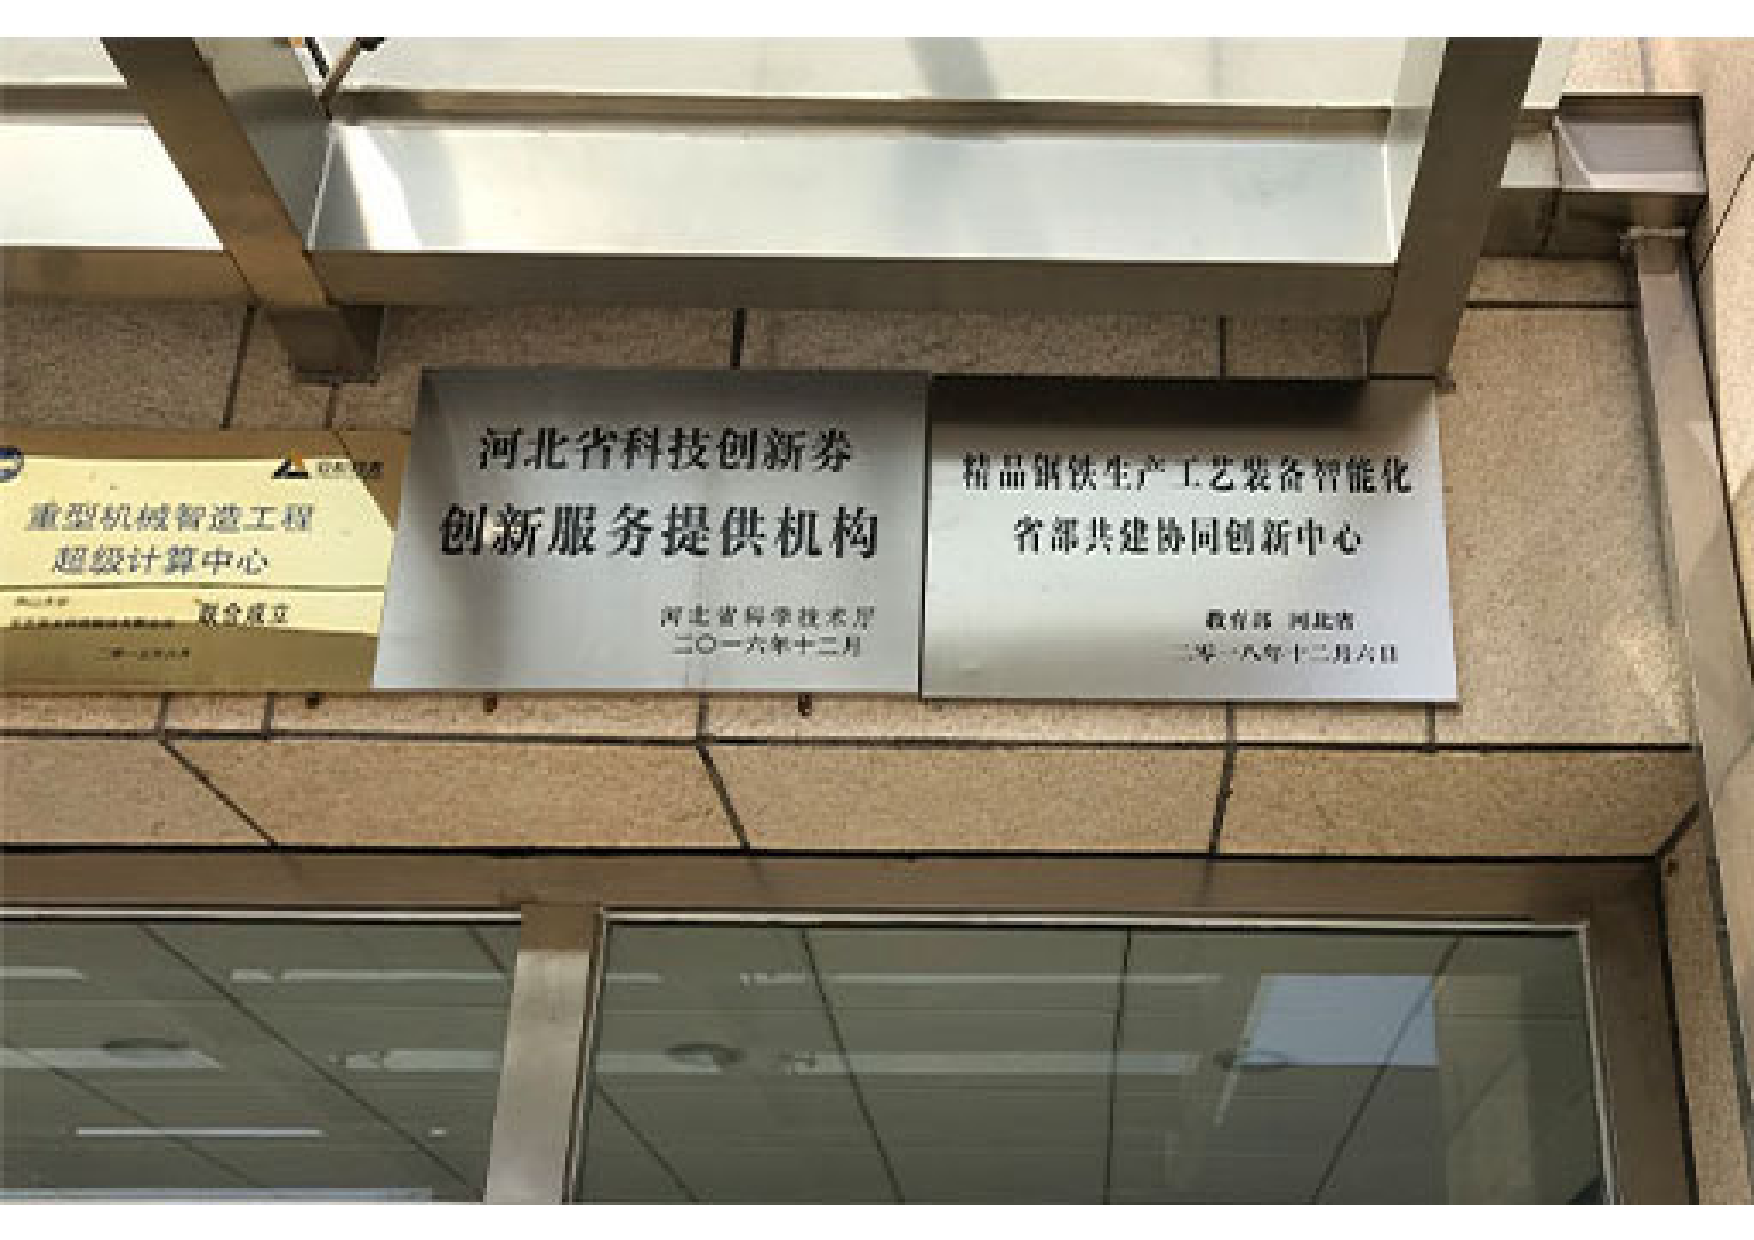
\includegraphics[width=0.4\textwidth]{精品钢铁生产工艺装备智能化省部共建协同创新中心.pdf}}
				\subcaptionbox{国家创新人才培养示范基地\label{fig_innovativetalents}}[0.49\textwidth]{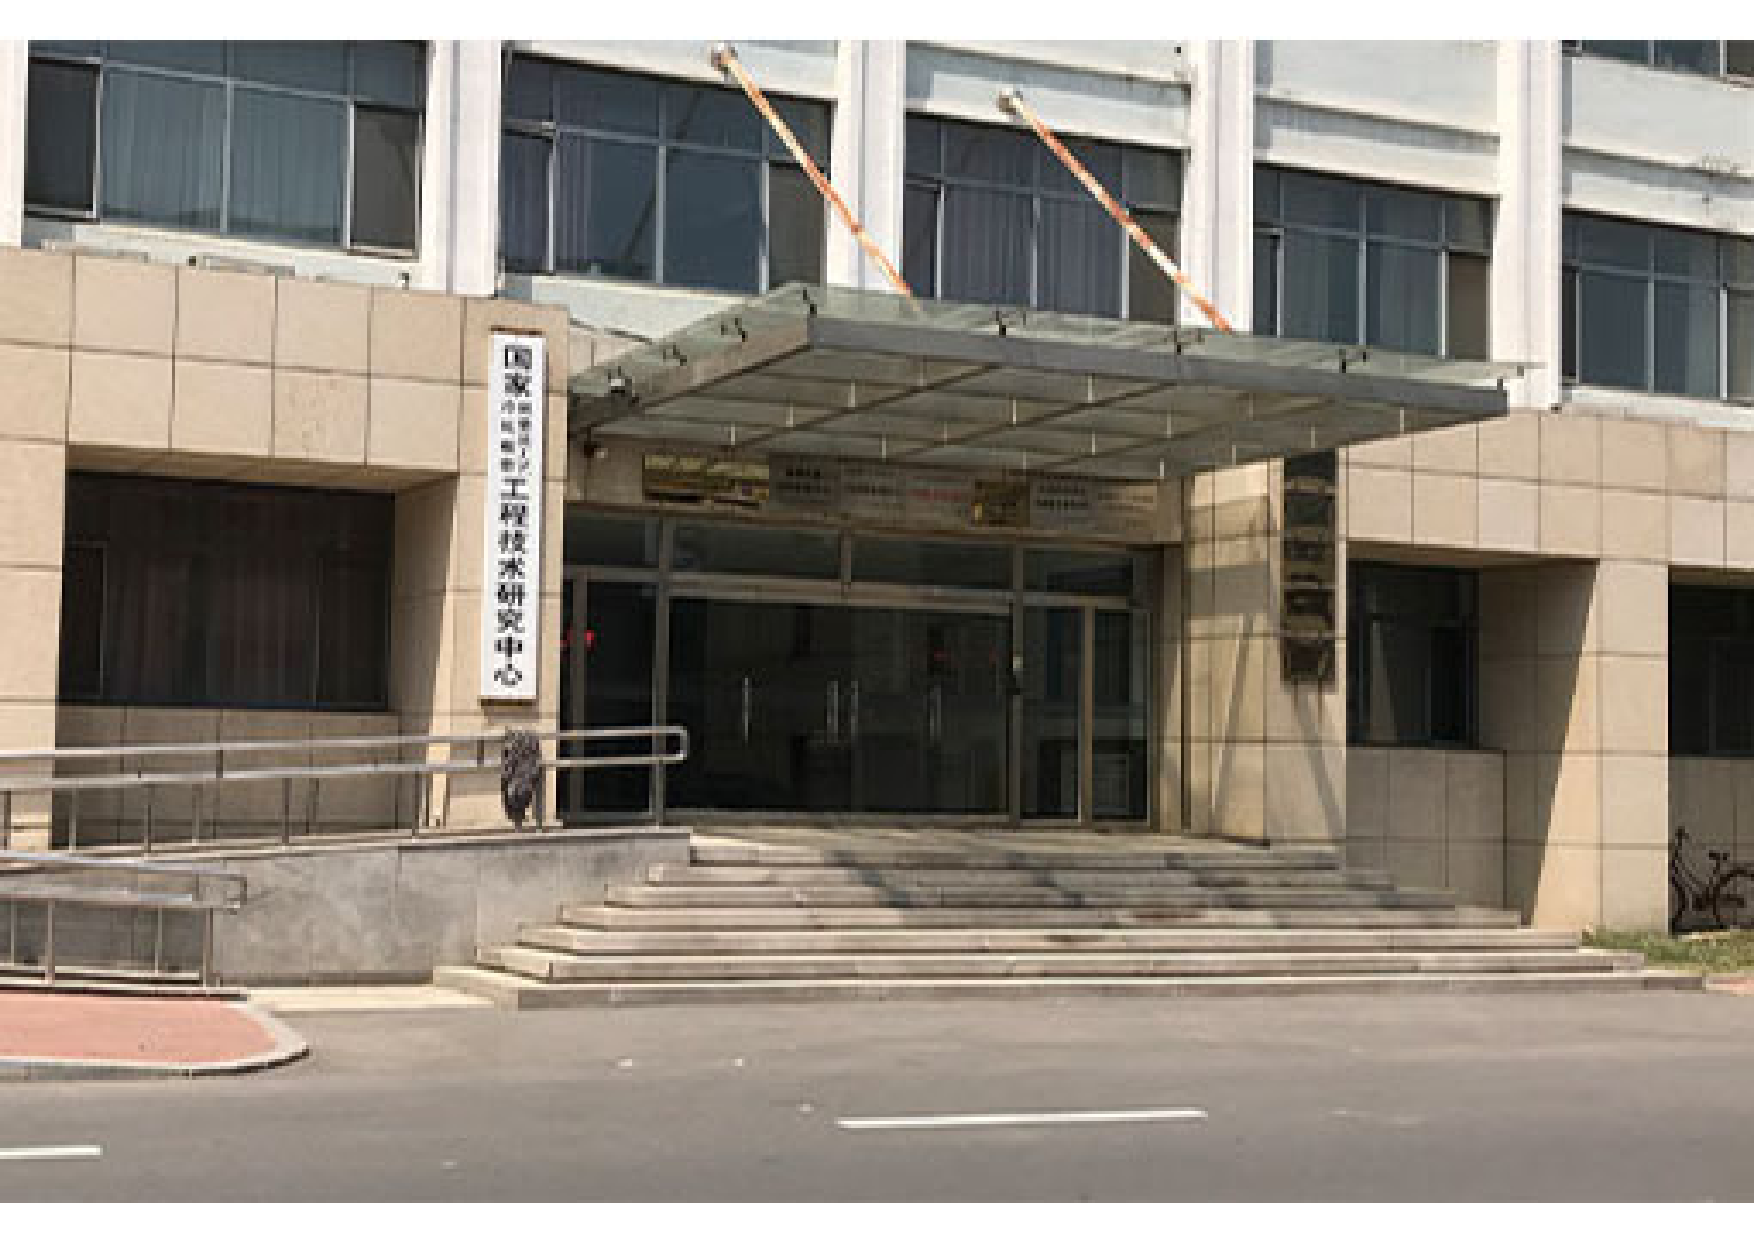
\includegraphics[width=0.4\textwidth]{国家创新人才培养示范基地.pdf}}
				\subcaptionbox{国家冷轧板带装备及工艺工程技术研究中心\label{fig_coldrolledstrip}}[0.49\textwidth]{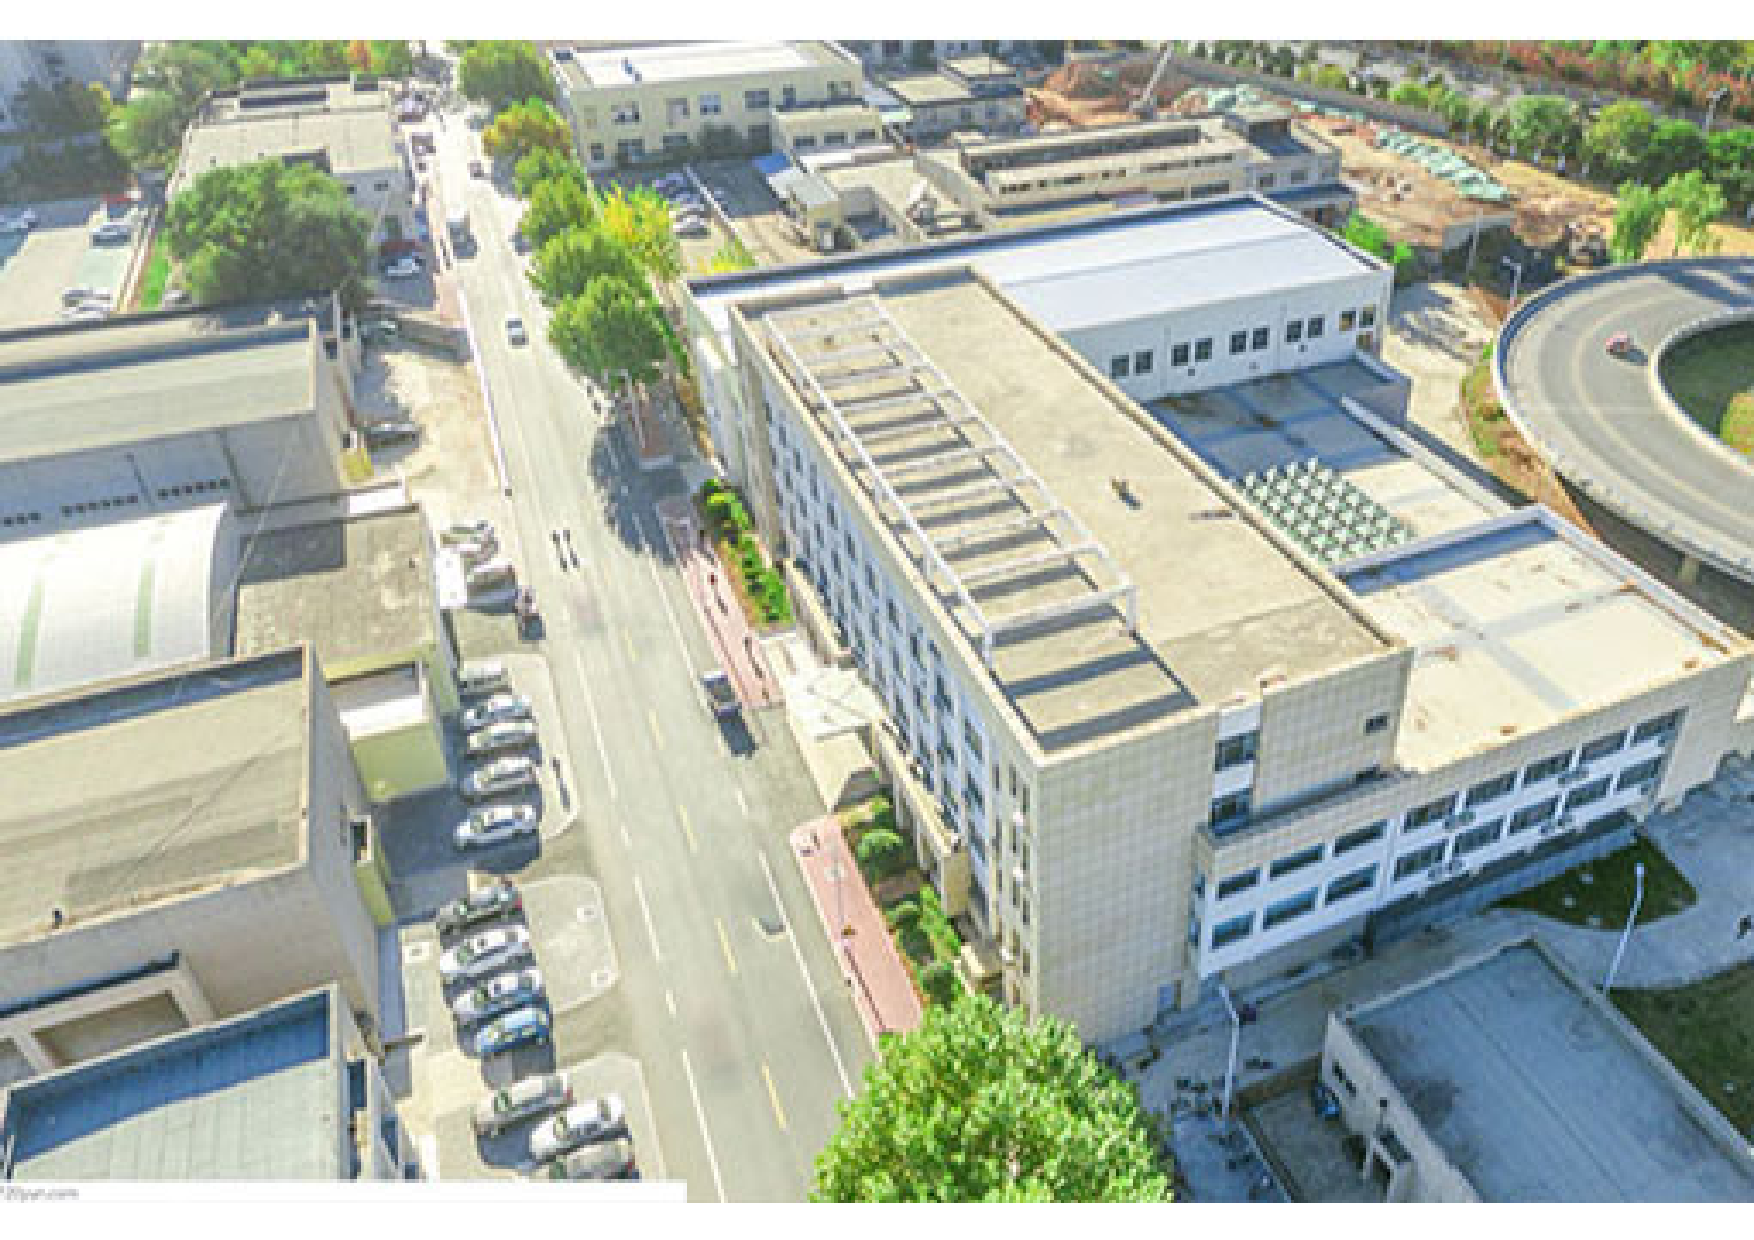
\includegraphics[width=0.4\textwidth]{国家冷轧板带装备及工艺工程技术研究中心.pdf}}
				\caption{燕山大学国家基地}
				\label{fig_ysunationalbase}
			\end{figure}
			
			\begin{figure}[!ht]
				\centering
				\bisubcaptionbox{亚稳材料制备技术与科学国家重点实验室\label{fig_bi_mmst}}{State Key Laboratory of Metastable Materials Science and Technology}[0.49\textwidth]{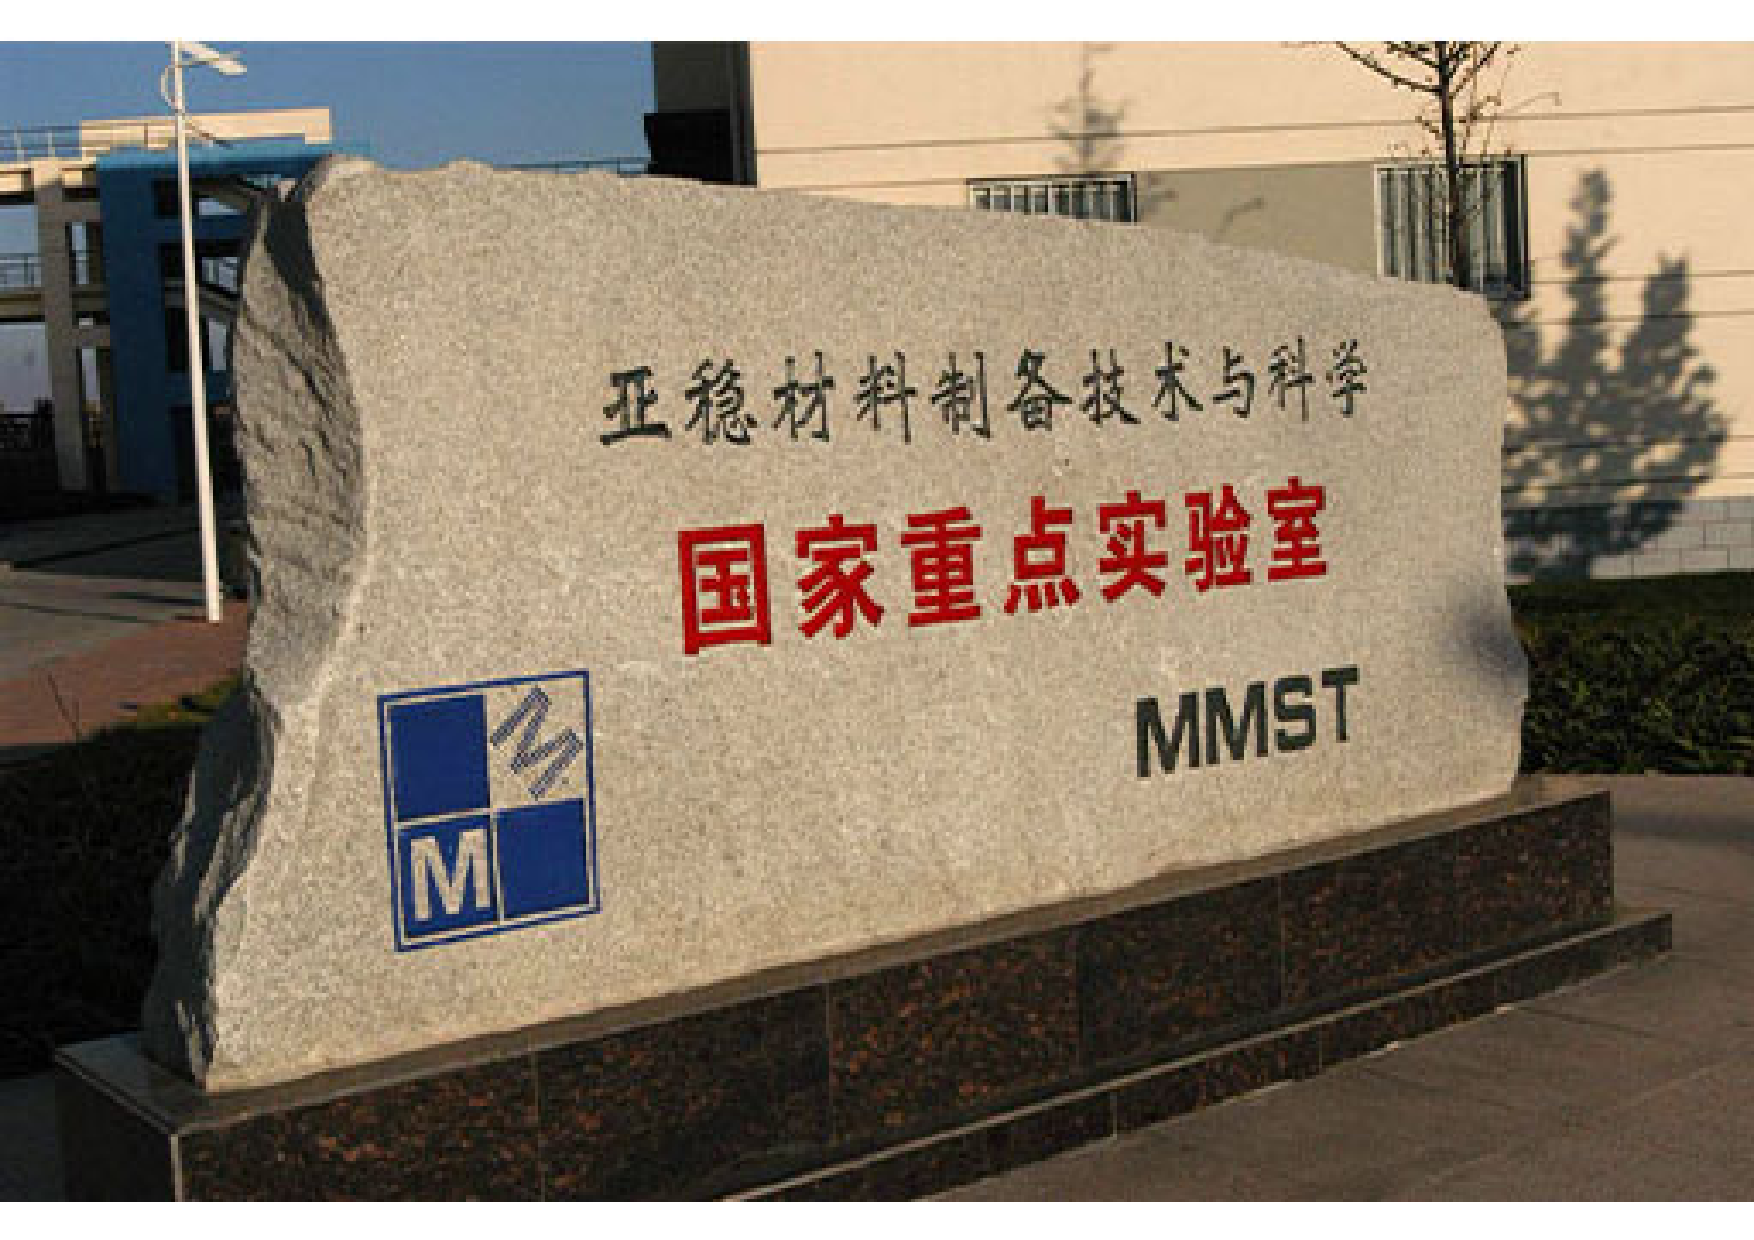
\includegraphics[scale=0.25]{亚稳材料制备技术与科学国家重点实验室.pdf}}
				\bisubcaptionbox{精品钢铁生产工艺装备智能化省部共建协同创新中心\label{fig_bi_finesteel}}{High-quality iron and steel production process equipment intelligence, the Ministry of Chemical Cooperation and Innovation Center}[0.49\textwidth]{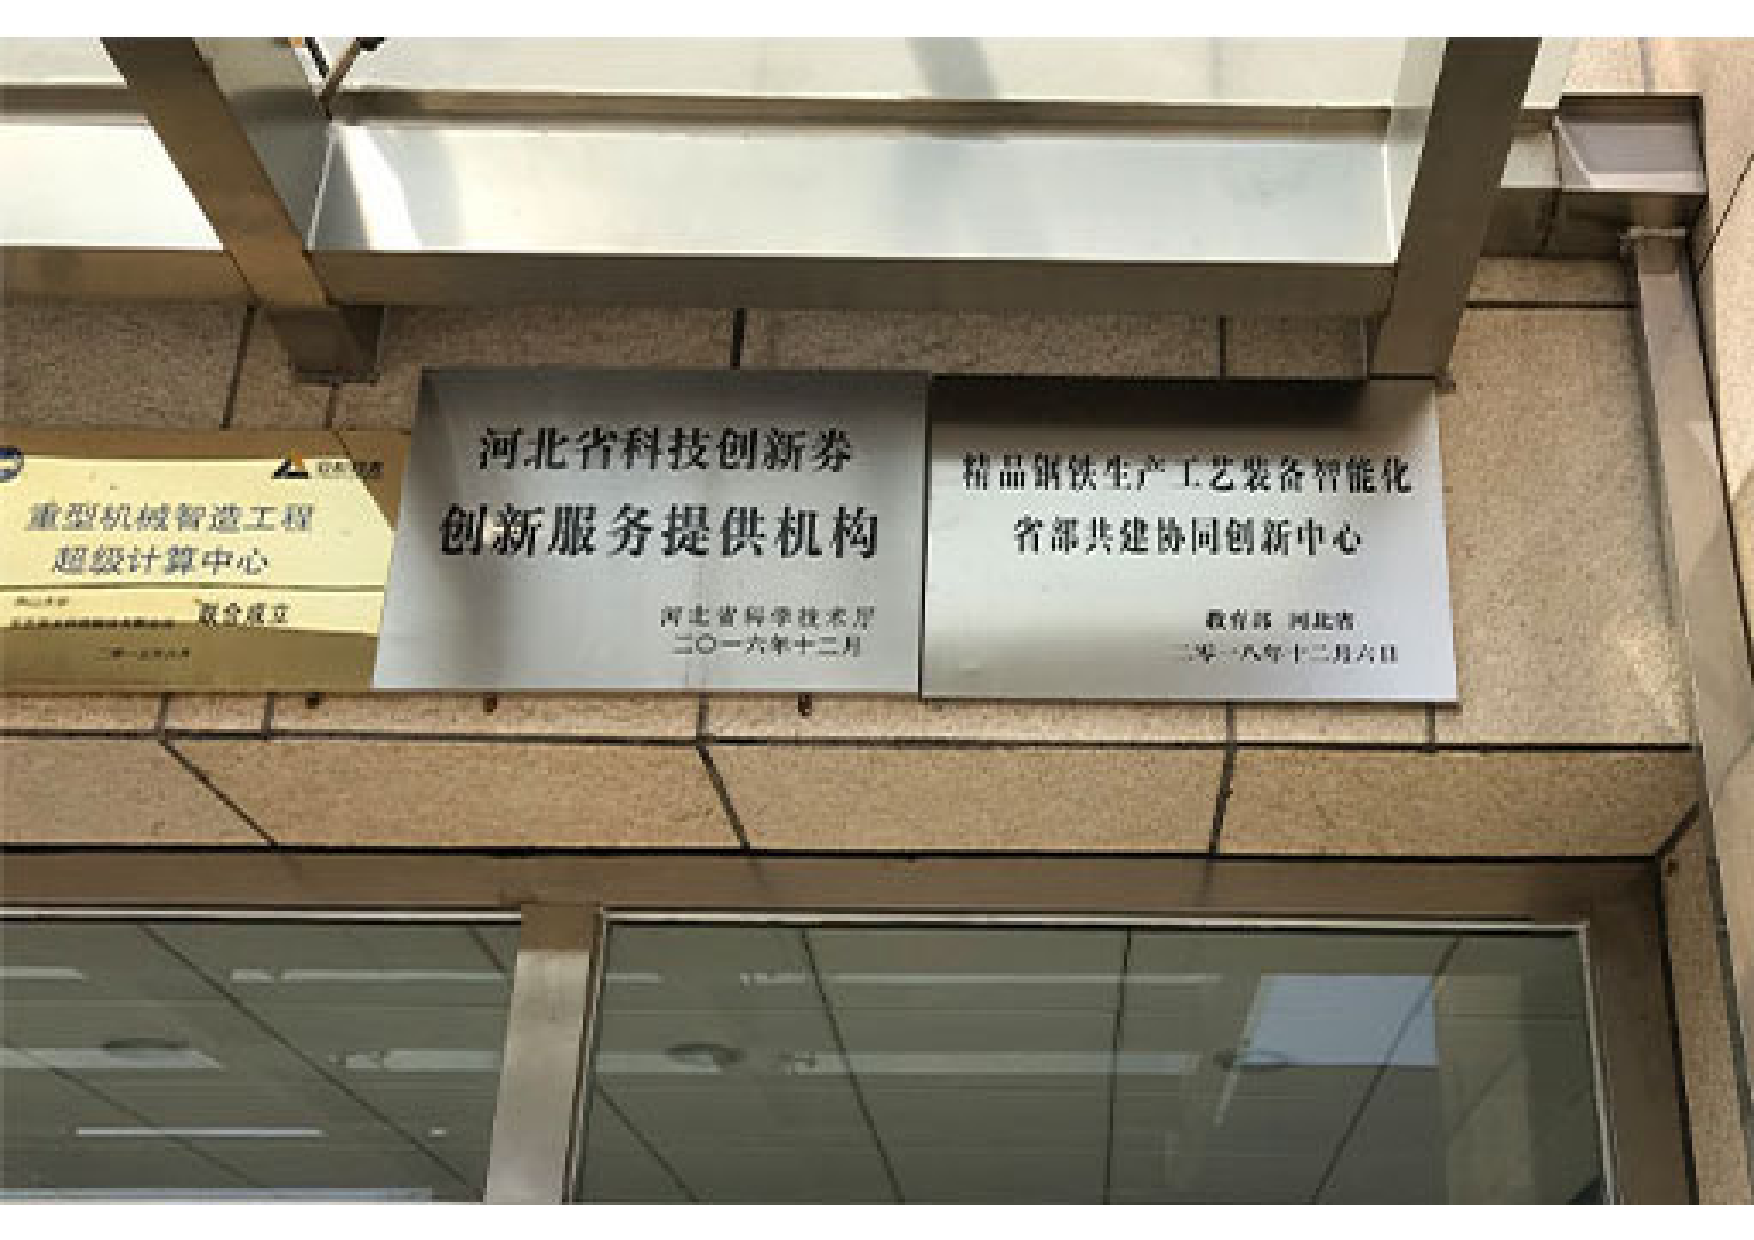
\includegraphics[scale=0.25]{精品钢铁生产工艺装备智能化省部共建协同创新中心.pdf}}
				\bisubcaptionbox{国家创新人才培养示范基地\label{fig_bi_innovativetalents}}{National Demonstration Base for training innovative talents}[0.49\textwidth]{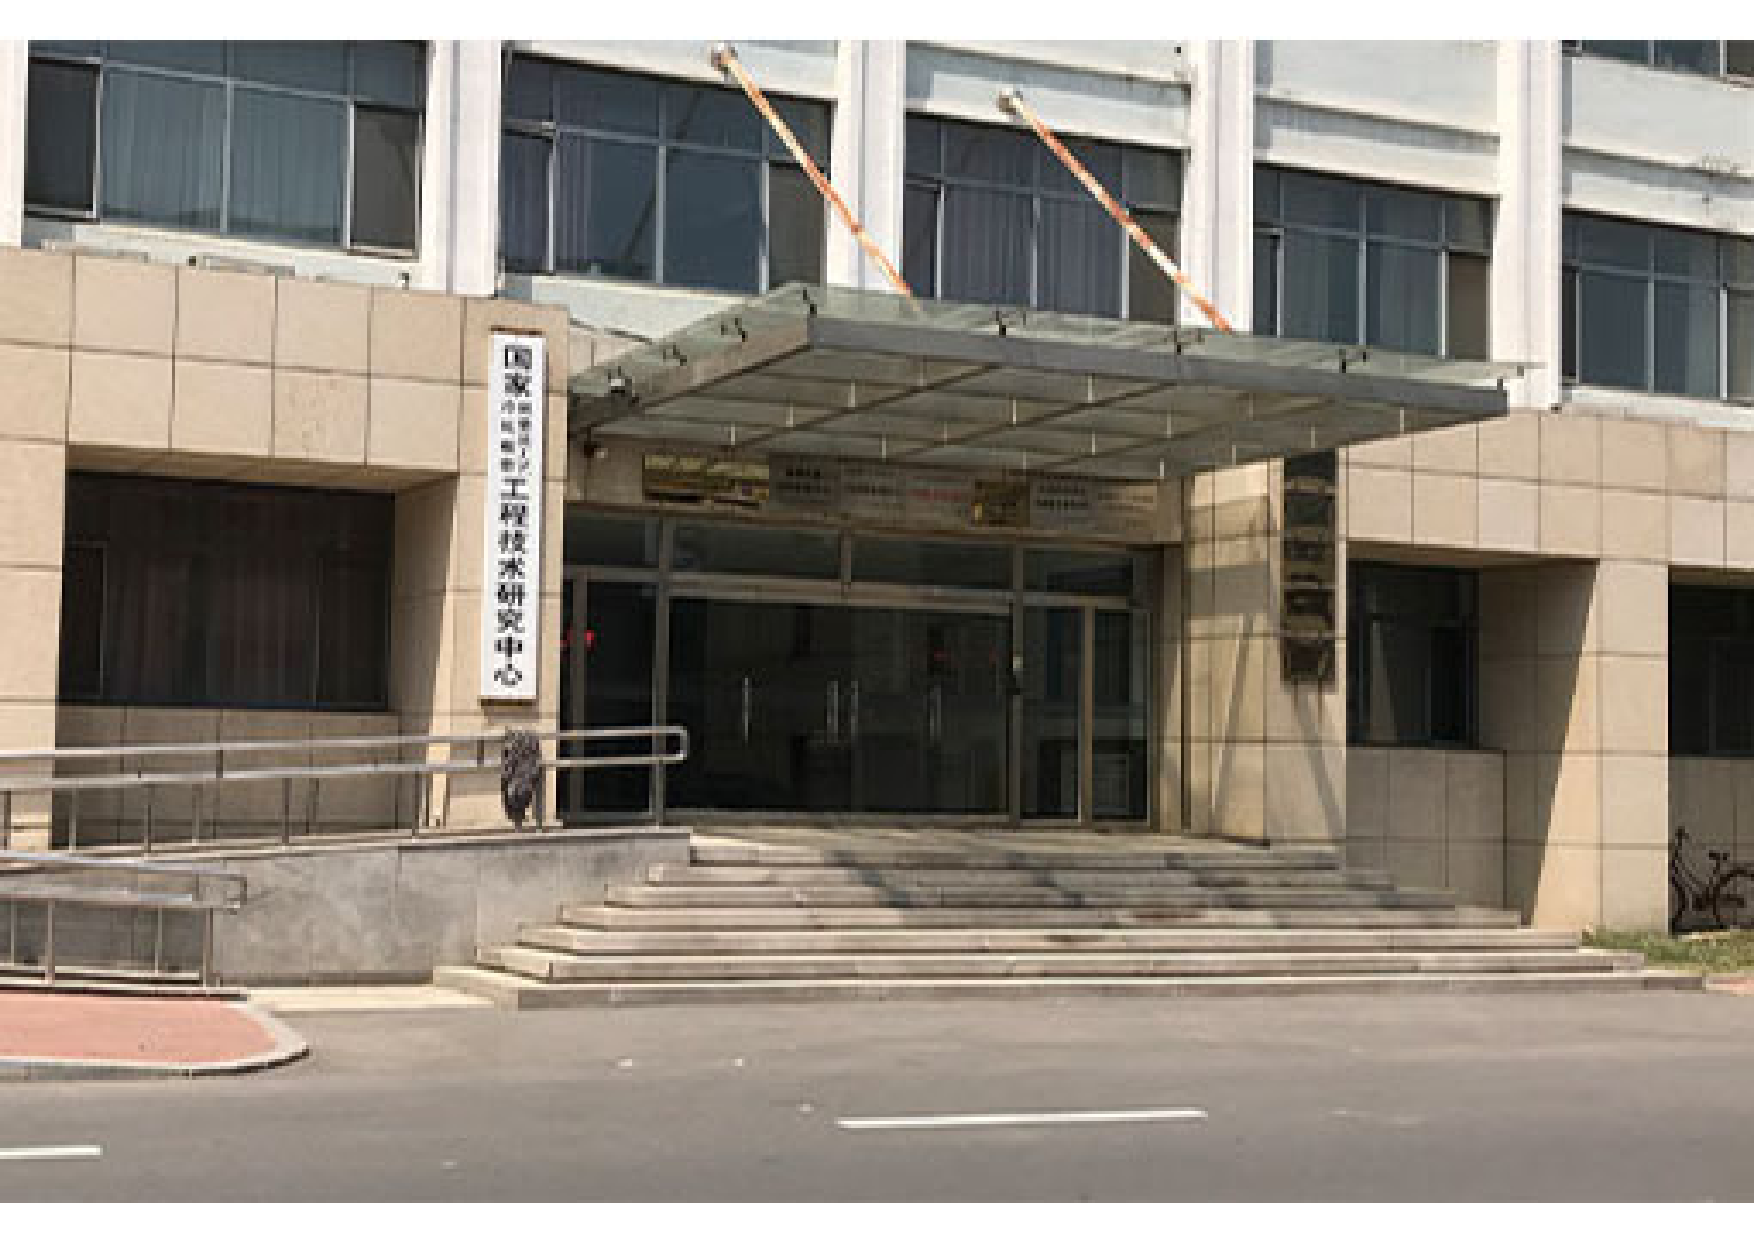
\includegraphics[scale=0.25]{国家创新人才培养示范基地.pdf}}
				\bisubcaptionbox{国家冷轧板带装备及工艺工程技术研究中心\label{fig_bi_coldrolledstrip}}{National Research Center for cold-rolled strip equipment and technology}[0.49\textwidth]{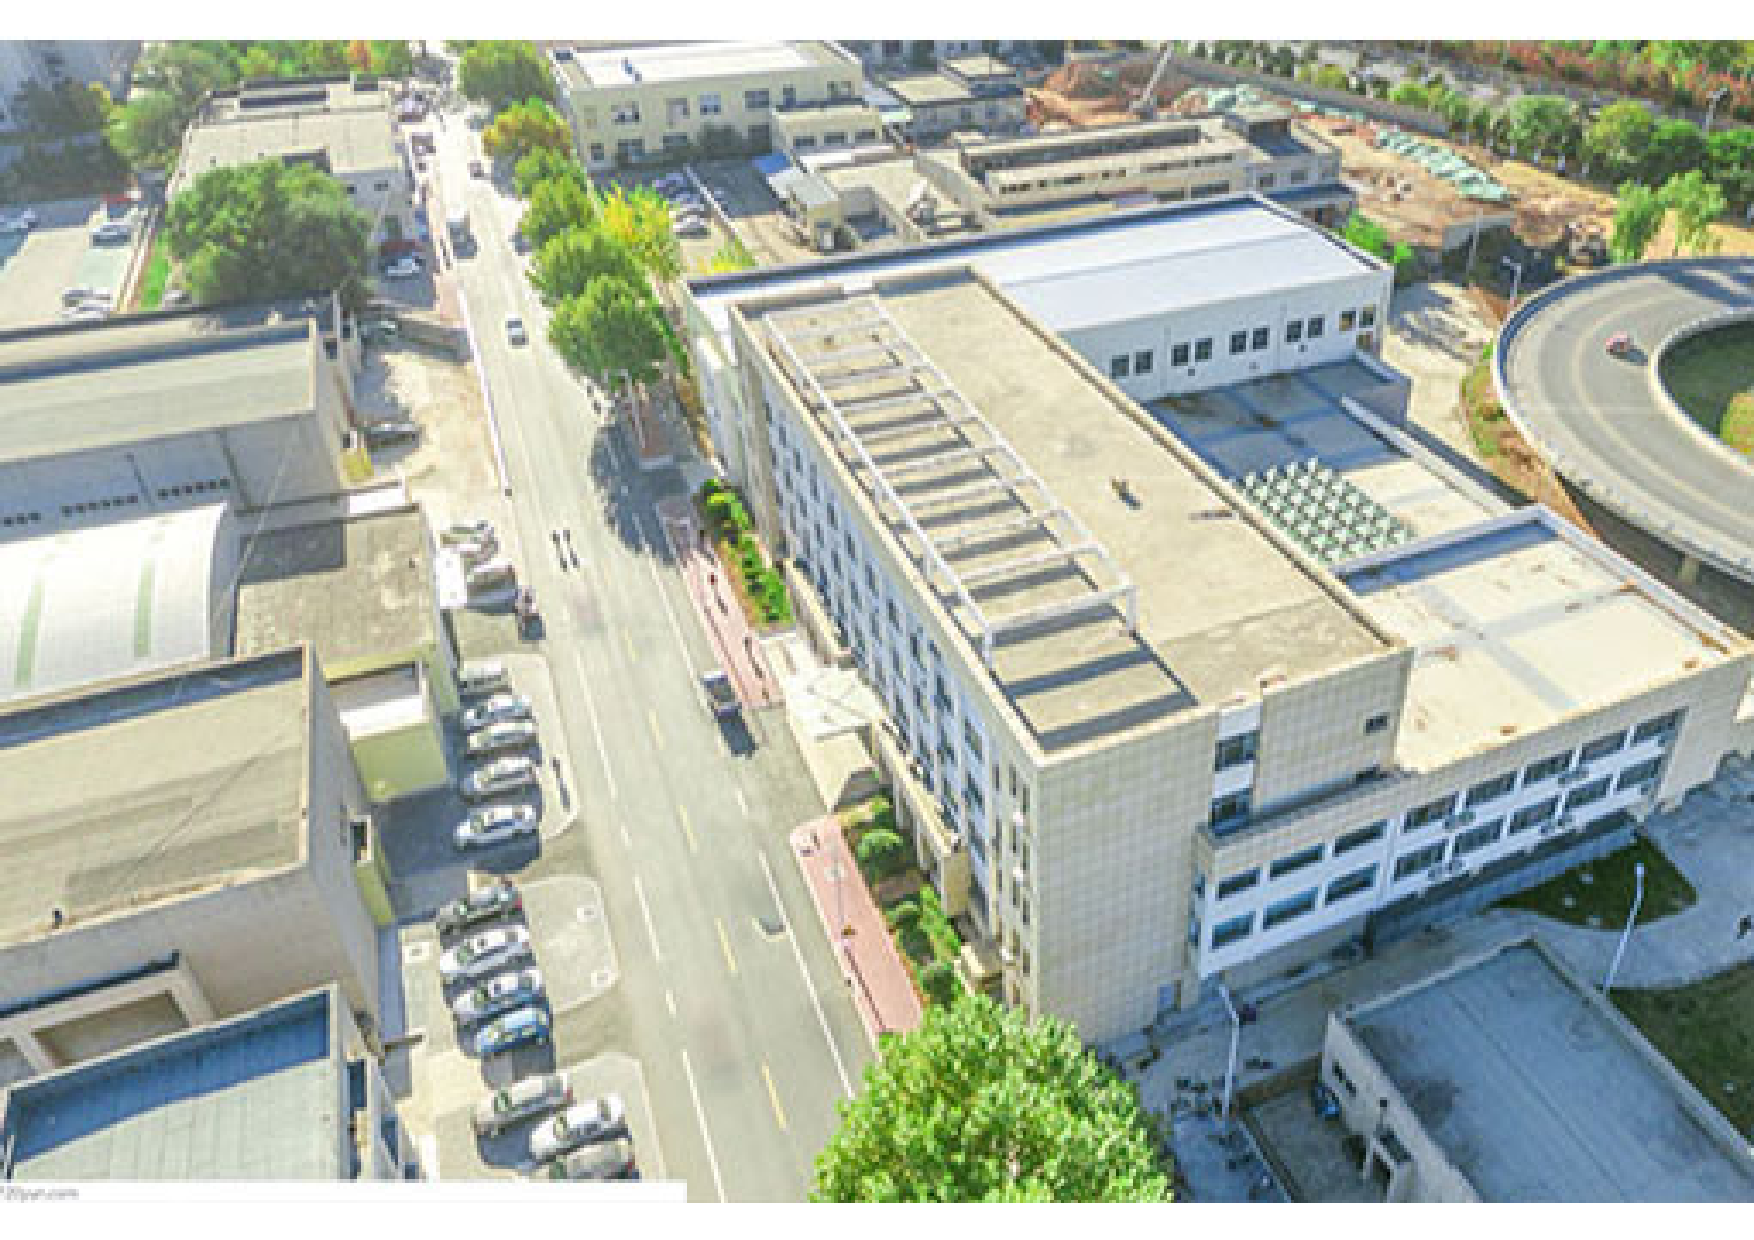
\includegraphics[scale=0.25]{国家冷轧板带装备及工艺工程技术研究中心.pdf}}
				\bicaption{燕山大学国家基地}{The national base of Yanshan University}
				\label{fig_bi_ysunationalbase}
			\end{figure}
		%-------------------插入多张图片示例结束-------------------


		三四五六七八九〇壹贰叁肆伍陆柒捌玖零一二三四五六七八九〇壹贰叁肆伍陆柒捌玖零一二三四五六七八九〇壹贰叁肆伍陆柒捌玖零一二三四五六七八九〇壹贰叁肆伍陆柒捌玖零一二三四五六七八九〇壹贰叁肆伍陆柒捌玖零一二三四五六七八九〇壹贰叁肆伍陆柒捌玖零一二三四五六七八九〇壹贰叁肆伍陆柒捌玖零一二三四五六七八九〇壹贰叁肆伍陆柒捌玖零一二三四五六七八九〇壹贰叁肆伍陆柒捌玖零

		三四五六七八九〇壹贰叁肆伍陆柒捌玖零一二三四五六七八九〇壹贰叁肆伍陆柒捌玖零一二三四五六七八九〇壹贰叁肆伍陆柒捌玖零一二三四五六七八九〇壹贰叁肆伍陆柒捌玖零一二三四五六七八九〇壹贰叁肆伍陆柒捌玖零一二三四五六七八九〇壹贰叁肆伍陆柒捌玖零一二三四五六七八九〇壹贰叁肆伍陆柒捌玖零一二三四五六七八九〇壹贰叁肆伍陆柒捌玖零一二三四五六七八九〇壹贰叁肆伍陆柒捌玖零
		
		三四五六七八九〇壹贰叁肆伍陆柒捌玖零一二三四五六七八九〇壹贰叁肆伍陆柒捌玖零一二三四五六七八九〇壹贰叁肆伍陆柒捌玖零一二三四五六七八九〇壹贰叁肆伍陆柒捌玖零一二三四五六七八九〇壹贰叁肆伍陆柒捌玖零一二三四五六七八九〇壹贰叁肆伍陆柒捌玖零一二三四五六七八九〇壹贰叁肆伍陆柒捌玖零一二三四五六七八九〇壹贰叁肆伍陆柒捌玖零一二三四五六七八九〇壹贰叁肆伍陆柒捌玖零
		
		三四五六七八九〇壹贰叁肆伍陆柒捌玖零一二三四五六七八九〇壹贰叁肆伍陆柒捌玖零一二三四五六七八九〇壹贰叁肆伍陆柒捌玖零一二三四五六七八九〇壹贰叁肆伍陆柒捌玖零一二三四五六七八九〇壹贰叁肆伍陆柒捌玖零一二三四五六七八九〇壹贰叁肆伍陆柒捌玖零一二三四五六七八九〇壹贰叁肆伍陆柒捌玖零一二三四五六七八九〇壹贰叁肆伍陆柒捌玖零一二三四五六七八九〇壹贰叁肆伍陆柒捌玖零

		下面是插入行内公式的示例。

		勾股定理$a^2+b^2=c^2$也被称为商高定理。

		下面是插入行间公式的示例。

		公式\eqref{eq:a^2+b^2}可以根据公式\eqref{eq:a}和\eqref{eq:b}得到。

		\begin{align}
			\theta&=\omega t\notag\\
			a&=\cos\theta \label{eq:a}\\
			b&=\sin\theta \label{eq:b}\\
			a^2+b^2&=1
			\label{eq:a^2+b^2}
		\end{align}

		式\eqref{eq2:a^2+b^2}可由式\eqref{eq2:identity_a_b}得出。
		\begin{subequations}
			\label{eq2:identity_a_b}
			\begin{align}
				\theta&=\omega t\notag\\
				a&=\cos\theta \label{eq2:a}\\
				b&=\sin\theta \label{eq2:b}\\
				a^2+b^2&=1
				\label{eq2:a^2+b^2}
			\end{align}
		\end{subequations}

		表\ref{tab_para1}~为插入表格示例。

		%--------------插表示例开始--------------
		\begin{table}[!ht]
			\caption{System Parameters}
			\label{tab_para1}
			\centering
			\begin{tabular}{CLR}
				\toprule
				Parameter & Description & Value \\
				\midrule
				$L$ & filter inductance & $2\mathrm{mH}$ \\
				$C$ & filter capacitance & $100\mu\mathrm{F}$ \\
				$R$ & load resistance & $10\Omega$ \\
				\bottomrule
			\end{tabular}
		\end{table}
		%--------------插表示例结束--------------
		\begin{table}[!ht]
			\bicaption{博士中文表题}{System Parameters}
			\label{tab_para2}
			\centering
			\begin{tabular}{CLR}
				\toprule
				Parameter & Description & Value \\
				\midrule
				$L$ & filter inductance & $2\mathrm{mH}$ \\
				$C$ & filter capacitance & $100\mu\mathrm{F}$ \\
				$R$ & load resistance & $10\Omega$ \\
				\bottomrule
			\end{tabular}
		\end{table}
		三四五六七八九〇壹贰叁肆伍陆柒捌玖零一二三四五六七八九〇壹贰叁肆伍陆柒捌玖零一二三四五六七八九〇壹贰叁肆伍陆柒捌玖零一二三四五六七八九〇壹贰叁肆伍陆柒捌玖零一二三四五六七八九〇壹贰叁肆伍陆柒捌玖零一二三四五六七八九〇壹贰叁肆伍陆柒捌玖零一二三四五六七八九〇壹贰叁肆伍陆柒捌玖零一二三四五六七八九〇壹贰叁肆伍陆柒捌玖零一二三四五六七八九〇壹贰叁肆伍陆柒捌玖零

		三四五六七八九〇壹贰叁肆伍陆柒捌玖零一二三四五六七八九〇壹贰叁肆伍陆柒捌玖零一二三四五六七八九〇壹贰叁肆伍陆柒捌玖零一二三四五六七八九〇壹贰叁肆伍陆柒捌玖零一二三四五六七八九〇壹贰叁肆伍陆柒捌玖零一二三四五六七八九〇壹贰叁肆伍陆柒捌玖零一二三四五六七八九〇壹贰叁肆伍陆柒捌玖零一二三四五六七八九〇壹贰叁肆伍陆柒捌玖零一二三四五六七八九〇壹贰叁肆伍陆柒捌玖零

		三四五六七八九〇壹贰叁肆伍陆柒捌玖零一二三四五六七八九〇壹贰叁肆伍陆柒捌玖零一二三四五六七八九〇壹贰叁肆伍陆柒捌玖零一二三四五六七八九〇壹贰叁肆伍陆柒捌玖零一二三四五六七八九〇壹贰叁肆伍陆柒捌玖零一二三四五六七八九〇壹贰叁肆伍陆柒捌玖零一二三四五六七八九〇壹贰叁肆伍陆柒捌玖零一二三四五六七八九〇壹贰叁肆伍陆柒捌玖零一二三四五六七八九〇壹贰叁肆伍陆柒捌玖零

		三四五六七八九〇壹贰叁肆伍陆柒捌玖零一二三四五六七八九〇壹贰叁肆伍陆柒捌玖零一二三四五六七八九〇壹贰叁肆伍陆柒捌玖零一二三四五六七八九〇壹贰叁肆伍陆柒捌玖零一二三四五六七八九〇壹贰叁肆伍陆柒捌玖零一二三四五六七八九〇壹贰叁肆伍陆柒捌玖零一二三四五六七八九〇壹贰叁肆伍陆柒捌玖零一二三四五六七八九〇壹贰叁肆伍陆柒捌玖零一二三四五六七八九〇壹贰叁肆伍陆柒捌玖零

	\chapter{第3章标题}

		三四五六七八九〇壹贰叁肆伍陆柒捌玖零一二三四五六七八九〇壹贰叁肆伍陆柒捌玖零一二三四五六七八九〇壹贰叁肆伍陆柒捌玖零一二三四五六七八九〇壹贰叁肆伍陆柒捌玖零一二三四五六七八九〇壹贰叁肆伍陆柒捌玖零一二三四五六七八九〇壹贰叁肆伍陆柒捌玖零一二三四五六七八九〇壹贰叁肆伍陆柒捌玖零一二三四五六七八九〇壹贰叁肆伍陆柒捌玖零一二三四五六七八九〇壹贰叁肆伍陆柒捌玖零

		三四五六七八九〇壹贰叁肆伍陆柒捌玖零一二三四五六七八九〇壹贰叁肆伍陆柒捌玖零一二三四五六七八九〇壹贰叁肆伍陆柒捌玖零一二三四五六七八九〇壹贰叁肆伍陆柒捌玖零一二三四五六七八九〇壹贰叁肆伍陆柒捌玖零一二三四五六七八九〇壹贰叁肆伍陆柒捌玖零一二三四五六七八九〇壹贰叁肆伍陆柒捌玖零一二三四五六七八九〇壹贰叁肆伍陆柒捌玖零一二三四五六七八九〇壹贰叁肆伍陆柒捌玖零

		三四五六七八九〇壹贰叁肆伍陆柒捌玖零一二三四五六七八九〇壹贰叁肆伍陆柒捌玖零一二三四五六七八九〇壹贰叁肆伍陆柒捌玖零一二三四五六七八九〇壹贰叁肆伍陆柒捌玖零一二三四五六七八九〇壹贰叁肆伍陆柒捌玖零一二三四五六七八九〇壹贰叁肆伍陆柒捌玖零一二三四五六七八九〇壹贰叁肆伍陆柒捌玖零一二三四五六七八九〇壹贰叁肆伍陆柒捌玖零一二三四五六七八九〇壹贰叁肆伍陆柒捌玖零

		表\ref{multipagetable}为跨页表格示例。
		\begin{longtable}{CC}
			\caption{Example Table}
			\label{multipagetable}\\
			\toprule
			第一列 & 第二列 \\
			\midrule
			\endfirsthead
			\multicolumn{2}{C}{表\thetable(续)}\\
			\toprule
			第一列 & 第二列 \\
			\midrule
			\endhead
			\bottomrule
			\endfoot
			一流课程建设等方面开展了深入交流 & Row 1, Column 2 \\
			Row 2, Column 1 & Row 2, Column 2 \\
			Row 3, Column 1 & Row 3, Column 2 \\
			Row 4, Column 1 & Row 4, Column 2 \\
			Row 5, Column 1 & Row 5, Column 2 \\
			Row 6, Column 1 & Row 6, Column 2 \\
			Row 7, Column 1 & Row 7, Column 2 \\
			Row 8, Column 1 & Row 8, Column 2 \\
			Row 9, Column 1 & Row 9, Column 2 \\
			Row 10, Column 1 & Row 10, Column 2 \\
			Row 11, Column 1 & Row 11, Column 2 \\
			Row 12, Column 1 & Row 12, Column 2 \\
			Row 13, Column 1 & Row 13, Column 2 \\
			Row 14, Column 1 & Row 14, Column 2 \\
			Row 15, Column 1 & Row 15, Column 2 \\
			Row 16, Column 1 & Row 16, Column 2
		\end{longtable}

		三四五六七八九〇壹贰叁肆伍陆柒捌玖零一二三四五六七八九〇壹贰叁肆伍陆柒捌玖零一二三四五六七八九〇壹贰叁肆伍陆柒捌玖零一二三四五六七八九〇壹贰叁肆伍陆柒捌玖零一二三四五六七八九〇壹贰叁肆伍陆柒捌玖零一二三四五六七八九〇壹贰叁肆伍陆柒捌玖零一二三四五六七八九〇壹贰叁肆伍陆柒捌玖零一二三四五六七八九〇壹贰叁肆伍陆柒捌玖零一二三四五六七八九〇壹贰叁肆伍陆柒捌玖零

		三四五六七八九〇壹贰叁肆伍陆柒捌玖零一二三四五六七八九〇壹贰叁肆伍陆柒捌玖零一二三四五六七八九〇壹贰叁肆伍陆柒捌玖零一二三四五六七八九〇壹贰叁肆伍陆柒捌玖零一二三四五六七八九〇壹贰叁肆伍陆柒捌玖零一二三四五六七八九〇壹贰叁肆伍陆柒捌玖零一二三四五六七八九〇壹贰叁肆伍陆柒捌玖零一二三四五六七八九〇壹贰叁肆伍陆柒捌玖零一二三四五六七八九〇壹贰叁肆伍陆柒捌玖零

	\section{本章小结}
		That's all for now!

	\chapter{结论}
		论文的结论部分是整个研究的归纳和总结,也是对研究问题的回答和对结果的解释。在这一部分中,研究者应该系统性地总结研究的主要发现,并就这些发现的意义进行讨论。同时,应该指出研究的局限性,并提出未来研究的方向。

		首先,结论部分应该对研究的核心发现进行简要总结,强调这些发现与研究问题之间的关系。然后,研究者需要讨论这些发现的意义,包括对理论、实践或政策的影响,并强调研究的贡献。此外,应该指出研究的局限性,即研究所面临的限制和可能存在的偏差,并提出改进方法。最后,结论部分应该提出未来研究的方向或建议,以便激发读者的兴趣,并为后续研究提供参考。

		总之,结论部分是整个论文的重要组成部分,需要深入总结研究的主要发现,并就这些发现的意义进行深入讨论,同时指出研究的局限性并提出未来研究的方向。

	\reference{ref.bib}

	\customizedappendix{
		%如无附录,可删除此部分内容。
		论文的附录通常包括一些额外的材料,用于补充和支持主体文本,但不适合直接放在正文中。以下是一些可能包含在附录中的内容。
		
		\begin{align}
			\theta&=\omega t\notag\\
			a&=\cos\theta \label{eq:appendix1_a}\\
			b&=\sin\theta \label{eq:appendix1_b}\\
			a^2+b^2&=1
			\label{eq:appendix1_a^2+b^2}
		\end{align}
		
		\begin{subequations}
			\label{eq2:appendix1_identity_a_b}
			\begin{align}
				\theta&=\omega t\notag\\
				a&=\cos\theta \label{eq2:appendix1_a}\\
				b&=\sin\theta \label{eq2:appendix1_b}\\
				a^2+b^2&=1
				\label{eq2:appendix1_a^2+b^2}
			\end{align}
		\end{subequations}
	}

	\customizedappendix{
		%如无附录,可删除此部分内容。
		论文的附录通常包括一些额外的材料,用于补充和支持主体文本,但不适合直接放在正文中。以下是一些可能包含在附录中的内容。
		
		\begin{align}
			\theta&=\omega t\notag\\
			a&=\cos\theta \label{eq:appendix2_a}\\
			b&=\sin\theta \label{eq:appendix2_b}\\
			a^2+b^2&=1
			\label{eq:appendix2_a^2+b^2}
		\end{align}
		
		\begin{subequations}
			\label{eq2:appendix2_identity_a_b}
			\begin{align}
				\theta&=\omega t\notag\\
				a&=\cos\theta \label{eq2:appendix2_a}\\
				b&=\sin\theta \label{eq2:appendix2_b}\\
				a^2+b^2&=1
				\label{eq2:appendix2_a^2+b^2}
			\end{align}
		\end{subequations}
	}


	\achievement{
		{\vspace{-0.1em}\noindent\textbf{\songtib\zihao{-4} 1.\enspace 发表的学术论文}\vspace{-0.41em}}    % 无学术论文时此项不必列出
		\begin{enumerate}[leftmargin=1.52em,itemsep=-0.4em,label={[\arabic*]}]\zihao{5}%%%%%%% 这一行的设定不要修改!!!
			\item ×××, ×××. 并联2-RRR/UPRR踝关节康复机器人机构及其运动学[J]. 机器人, 2010, 32(1): 6-12. (EI收录号: 20101212786168)
			\item ×××, ×××. 空间并联机构连续刚度非线性映射研究[J]. 机械工程学报, 2008, 44(8): 20-25. (EI收录号: 083911606237)
			\item ×××, ×××. A sampling robot for high dust and strong corrosion environment[C]//International Conference on Robotic and Biomimetics, Tianjin, 2010: 828-832. (EI收录号: 20111313856140)
			\item ×××, ×××. 双重驱动四自由度并联机构型综合[J]. 机械设计与研究, 2008, 24(1): 51-53.
			\item $\cdots$要与参考文献格式一致!!!
		\end{enumerate}

		%%%%%%%%%%%%%%%%%%%%%%%%%%%%%%%%%%%%%%%%%%%%专著/译著
		{\vspace{-0.44em}\noindent\textbf{\songtib\zihao{-4} 2.\enspace 发表的专著/译著(无著作时此项不必列出)}\vspace{-0.41em}}    % 无专著/译著时此项不必列出
		\begin{enumerate}[leftmargin=1.52em,itemsep=-0.4em,label={[\arabic*]}]\zihao{5}%%%%%%% 这一行的设定不要修改!!!
			\item ×××, ×××. 高等空间机构学 [M]. 北京: 机械工业出版社, 2010.
			\item ×××, ×××. 空间并联机构导论 [M]. ×××, 译. 秦皇岛: 燕山大学出版社, 2020.
		\end{enumerate}

		%%%%%%%%%%%%%%%%%%%%%%%%%%%%%%%%%%%%%%%%%%%%%%%%%%%%%%%%%%%%%%%%%%%%%%%%%%%%%%%%%%%%%%
		{\vspace{-0.44em}\noindent\textbf{\songtib\zihao{-4} 3.\enspace 申请及已获得的专利(无专利时此项不必列出)}\vspace{-0.41em}}    % 无专利时此项不必列出
		\begin{enumerate}[leftmargin=1.52em,itemsep=-0.4em,label={[\arabic*]}]\zihao{5}%%%%%%% 这一行的设定不要修改!!!
			\item ×××, ×××. 具有远程运动中心的三自由度转动并联机构: 中国, 200910073844.8 [P]. 2011-01-05.
			\item ×××, ×××. 五自由度双重驱动并联机构: 中国, 200910075071.7 [P]. 2011-01-05.
		\end{enumerate}

		%%%%%%%%%%%%%%%%%%%%%%%%%%%%%%%%%%%%%%%%%%%%%%%%%%%%%%%%%%%%%%%%%%%%%%%%%%%%%%%%%%%%%%
		{\vspace{-0.44em}\noindent\textbf{\songtib\zihao{-4} 4.\enspace 科研获奖(无奖励时此项不必列出)}\vspace{-0.41em}}    % 无奖励时此项不必列出
		\begin{enumerate}[leftmargin=1.52em,itemsep=-0.4em,label={[\arabic*]}]\zihao{5}%%%%%%% 这一行的设定不要修改!!!
			\item ×××, ×××. 机器人机型综合及结构分析理论. XX省科学技术二等奖, 2009.
		\end{enumerate}
	}

	\acknowledgement{
		本论文的顺利完成,离不开导师XXX老师的悉心指导和教诲。在研究过程中,导师给予了我充分的自由空间和宝贵的建议,让我受益匪浅。

		同时,我要感谢实验室的师兄师姐们,他们在实验设备的使用和数据分析方面给予了我大量的帮助。他们的热情和支持让我在科研道路上走得更远。

		最后,我要特别感谢我的家人。是他们的无私支持和理解,让我能够全身心地投入到研究工作中,顺利完成了这篇论文。
	}

\end{document}
